\documentclass[12pt, a4paper]{report}
\usepackage[utf8]{inputenc}
\usepackage{ucs}
\usepackage[croatian]{babel}
\usepackage[margin=1.4in]{geometry}
\usepackage[labelsep=period]{caption}
\usepackage{graphicx}
\usepackage{amsthm}
\usepackage{amssymb}
\usepackage{afterpage}
\usepackage{amsmath}
\usepackage{mathtools}
\usepackage{epstopdf}
\usepackage{array}
\usepackage{epigraph}
\usepackage{tikz}
\usepackage[chapter]{algorithm}  
\usepackage{algorithmic}
\usepackage{color, colortbl}
\usetikzlibrary{trees}
\usepackage{setspace}
\usepackage{hyperref}
\usepackage{listings}
\usepackage{multirow}
\usepackage{booktabs}
\usepackage[titletoc,page]{appendix}
\usepackage{fancyhdr}
\usepackage{fancyvrb} 
\def\signed #1{{\leavevmode\unskip\nobreak\hfil\penalty50\hskip2em
		\hbox{}\nobreak\hfil(#1)%
		\parfillskip=0pt \finalhyphendemerits=0 \endgraf}}


\hypersetup{
	colorlinks,
	citecolor=black,
	filecolor=black,
	linkcolor=black,
	urlcolor=black
}

\setlength{\epigraphwidth}{.7\textwidth}
\usepackage{etoolbox}
\makeatletter
\patchcmd{\@makechapterhead}% <cmd>
{\thechapter}% <search>
{\thechapter.}% <replace>
{}{}% <success><failure>
\renewcommand{\@seccntformat}[1]{\csname the#1\endcsname.\quad}
\makeatother
\let\oldthebibliography\thebibliography
\let\endoldthebibliography\endthebibliography
\renewenvironment{thebibliography}[1]{
	\begin{oldthebibliography}{#1}
		\setlength{\itemsep}{0.27em}
		\setlength{\parskip}{0.27em}
	}
	{
	\end{oldthebibliography}
}


\addto\captionscroatian{%
\def\refname{Literatura}%
\def\bibname{Literatura}%
\def\tablename{Tabela}%
}%
\definecolor{mygreen}{rgb}{0,0.6,0}
\definecolor{mygray}{rgb}{0.5,0.5,0.5}
\definecolor{mymauve}{rgb}{0.58,0,0.82}


\definecolor{Gray}{gray}{0.7}
\definecolor{LightGray}{gray}{0.9}

\theoremstyle{definition}
\newtheorem{mydef}{Definicija} [chapter]
\newtheorem{myexp}{Primjer} [chapter]
\newtheorem{myteo}{Teorem} [chapter]
\newtheorem{mypro}{Dokaz} [chapter]
\makeatletter
\newcommand{\newalgname}[1]{%
	\renewcommand{\ALG@name}{#1}%
}

\renewcommand{\tablename}{Tabela}
\newalgname{Algoritam}
\renewcommand{\listalgorithmname}{Lista\ALG@name s}
\makeatother
\newcolumntype{g}{>{\columncolor{LightGray}}m}

\tikzstyle{level 1}=[level distance=3.5cm, sibling distance=3.5cm]
\tikzstyle{level 2}=[level distance=3.5cm, sibling distance=2.5cm]
\tikzstyle{igrac} = [text width=4.5em, text centered,top color =red!20, bottom color=red!20]
\tikzstyle{end} = [rectangle, minimum width=3pt,fill, inner sep=0pt, top color =blue, bottom color=blue, text centered, draw ]

%opening
\title{Document Managment System}
\author{Šeila Bećirović}


\begin{document}
\begin{titlepage}
	\newcommand{\HRule}{\rule{\linewidth}{0.55mm}} 
	\noindent
	{\large
		\begin{minipage}{0.2\textwidth}
			\begin{center} 
				
\includegraphics[width=0.7\textwidth]{unsa.jpg}
			\end{center}
		\end{minipage}
		\begin{minipage}{0.58\textwidth}
			\begin{center} \large
				Univerzitet u Sarajevu\\
				Elektrotehnički fakultet u Sarajevu\\
				Odsjek za računarstvo i informatiku\\
			\end{center}
		\end{minipage}
		\begin{minipage}{0.2\textwidth}
			\begin{center} 
				
\includegraphics[width=0.7\textwidth]{ETF_logo.png}
			\end{center}
		\end{minipage}
		\\[5 cm] 
		
		
		\begin{center}
		\LARGE 
		\bfseries 
		Database handler \& meta data visualizer \\[0.5cm]
		
		
		\LARGE
		Baze podataka \\[4cm]
		
		\end{center}		 		

		
		\begin{minipage}{0.45\textwidth}
			\begin{flushleft}
				\emph{Mentor}: \\
				Doc. dr. Emir Buza \\
			\end{flushleft}
		\end{minipage}
		~
		\begin{minipage}{0.04\textwidth}
			\begin{flushleft}
				
			\end{flushleft}
		\end{minipage}
		~
		\begin{minipage}{0.45\textwidth}
			\begin{flushright}
				\emph{Studenti}: \\
				Bećirović Šeila\\
				Džirlo Timur\\
				Pejčinović Dario
			\end{flushright}
		\end{minipage}\\[0.7 cm]
		
		\begin{center}
			{\large Sarajevo, 05.11.2017.}\\[1cm] 
		\end{center}
		\normalsize
		
		\vfill 
	}
\end{titlepage}
\renewcommand{\chaptermark}[1]{\markboth{#1}{}}
\lhead{}

\newpage
\begin{spacing}{0.9}
	\tableofcontents
\end{spacing}
\pagenumbering{arabic}
\chapter{Opis teme}

Namjena database handler-a i meta data visualizer-a jeste sama analiza Oracle baze podataka koja postoji na fakultetu, te pretvaranje gomile meta podataka u razumljivu formu koja može dati dosta korisnih informacija. Pod tim se također podrazumijeva i vizualizacija strukture same baze podataka kao i objekata koji su pohranjeni u istoj. Omogućene su izmjene procedura, trigera, odnosno svih objekata baze. Pored izmjena, omogućeno je i dodavanje i brisanje istih, te pregled podataka baze i dodavanje, brisanje i izmjena podataka baze.

\section{Funkcionalnosti sitema DHMV}


Funkcionalnosti sistema su podijeljene u dvije kategorije: upravljanje bazom i vizualizacija meta data. Vizualizacija meta data omogućava korisniku da vidi odgovarajuće podatke o bazi, o svojoj bazi, odnosno vrši prevođenje istih u oblik razumljiv korisniku, a upravljanje omogućava uređivanje objekata, tabela, itd.

\begin{itemize}
	\item Pregled svih baza podataka;
	\item Pregled svih tabela baze podatka;
	\item Upravljanje objektima vezanih za bazu i tabele;
	\item Pregled svih korisnika baze podataka;
	\item Vizualizacija meta podataka;
	\item Prikaz, kreiranje, uređivanje i brisanje podataka unutar baze.
\end{itemize}

U nastavku je prikazan dijagram slučajeva upotrebe.

\begin{figure}
		\begin{center} 
			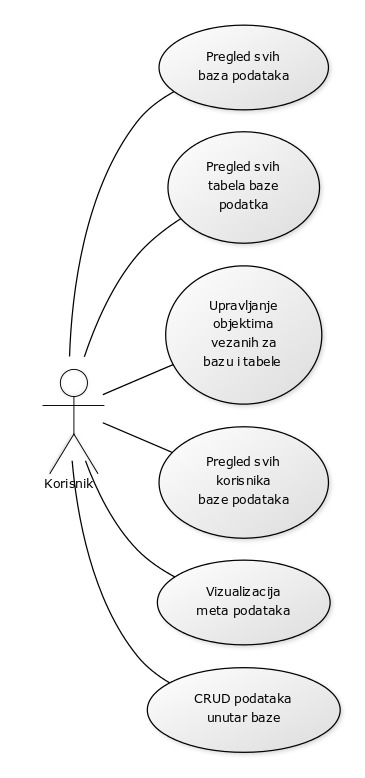
\includegraphics[width=0.7\textwidth]{usecase.jpg}
		\end{center}
\end{figure}




\chapter{Detaljni opis funkcionalnosti}


U ovom poglavlju su detaljno opisane funkcionalnosti aplikacije. Poslovni procesi koji se ostvaruju kroz ovu aplikaciju jesu vizualizacija metapodataka i ostalih relevantnih informacija o organizaciji baze, shemi baze, objektima i slično. Pod pojmom baze podataka u ovom radu smatra se jedna baza podataka nekog sistema kojima je moguće pristupiti kroz jednu konekciju, a ne skupa baza podataka. Svim funkcionalnostima ove aplikacije se pristupa  pomoću grafičkog okruženja. Prije svega, korisnik aplikaciji pristupa unosom korisničkog računa i lozinke (ovom procesu podliježe validacija unesenih vrijednosti). 

\section{Pregled svih baza podataka}
Nakon uspješne prijave na aplikaciju, korisniku se prikazuje lista svih baza koje se nalaze na jednom sistemu. O svim bazama su date informacije njihovih vlasnika i vremena kreiranja. Dalje se korisniku omogućava odabir pojedinačne baze podataka u svrhu pribavljanja detaljinih informacija koje su relevantne korisniku. Pod tim informacijama se smatraju informacije o objektima kao što su tabele, objekti, itd. 

\section{Pregled svih tabela baze podataka}
Nakon što korisnik odabere željenu bazu podataka, prikazuju se sve tabele koje se nalaze u odabranoj bazi podataka. Podaci koji se prikazuju pored naziva tabele su nazivi kolona, ograničenja nad kolonama, primarnom i sekundarnom ključu i informacija o tipu podatka i veličine kolone. Pored navedenog, korisnik će moći odabrati tabelu u svrhu otkrivanja većeg skupa informacija nad samom tabelom. Relevantne informacije koje će korisnik moći prikupiti ovom funkcionalnosti su opisane u nastavku teksta. 
Pored mogućnosti za odabirom željenih objekata, korisnik će moći pristupiti podacima koje se nalaze u tabeli. Nad tako prikuljenim podacima neće biti omogućeno njihova izmjena radi sigurnosti i konzistentnosti podataka. Podaci će biti prikazani u formi lakše razumljivoj čovjeku, odnosno pomoću tabele.

\section{Upravljanje objektima vezanih za bazu i/ili tabelu}
Nakon odabira tabele, korisniku se prikazuju svi kreirani objekti koji su vezani za nju. Pod objektima se smatraju indeksi, funkcije, trigeri, pogledi, greške i sekvence. Prikazani podaci će biti kategorizirani te će biti omogućen pristup  svakom objektu u cilju pregleda, izmjene ili brisanja istog. Rad nad objektima će se vršiti putem grafičkog interfejsa. Unutar ove funkcionalnosti se podrazumijeva:
	\begin{itemize}
		\item Kreiranje objekata baze;		
		\item Kreiranje tabela;
		
		\item Kreiranje pogleda;
		
		\item Kreiranje procedura;
		
		\item Kreiranje  trigera;
		
		\item Kreiranje PL/SQL, source objekata;
		
		\item Prikaz ERD baze.
	\end{itemize}

\section{Pregled svih korisnika baze podataka}
Ovaj poslovni proces omogućava pribavljanje informacije o svim korisnicima baze podataka. O nima će se dati pregled broja kreiranih objekata, baza podataka nad kojim imaju privilegije te ostalim relevantnim informacijama koje će dati pobliži uvid u informacije o pojedinom korisniku.
\newpage
\section{Vizualizacija meta podataka}
Vizualizacija meta podataka omogućava korisniku pregled svih informacija o samoj bazi podataka, koji su prevedeni na jezik razumljiv korisniku.
Obuhvata:
\begin{itemize}
\item 	Pregled svih objekata baze;

\item Pregled svih tabela;

\item Pregled svih pogleda;

\item Pregled svih argumenata funkcija i procedura;

\item Pregled svih procedura;

\item Pregled svih trigera;

\item Pregled svih PL/SQL, source objekata;
\item Prikaz ERD baze.
\end{itemize}
\section{Prikaz, kreiranje, uređivanje i brisanje podataka unutar baze}
Data funkcionalnost omogućava korisniku da vidi podatke u tabelama baze, te da dodaje nove redove, uređuje i briše postojeće redove.

\chapter{Tehnologija}

Stack \footnote{Stack - izraz koji se u IT svijetu koristi da opiše skupinu softverskih komponenti koje kao takve tvore platformu na kojoj će funkcionisati određena aplikacija ili skupina aplikacija. Neki od poznatijih tehnoloških Stack-ova su WAMP ( Windows Apache MySQL PHP) i LAMP ( Linux Apache MySQL PHP)}  tehnologija koji je odabran za implementaciju ove web aplikacije se sastoji iz:
\begin{itemize}
	\item Java Spring - back-end;
	\item AngularJS - front-end;
	\item PostgreSQL - interna baza podataka;
	\item OracleDB - baza podataka koja se analizira;
	\item Android SDK.
\end{itemize}

U nastavku će biti pojedinačno opisane tehnologije, kao i motivacija za njihovo korištenje.

\section{Java Spring}
Java Spring predstavlja aplikacijski framework za razvoj poslovnih aplikacija(engl. enterprise application) korištenjem Java programskog jezika koji podržava višenamjensko programiranje i striktno definisan konfiguracijski model, nezavisan od produkcijske platforme. Spring obezbjeđuje posebnu podršku za razvoj web aplikacija i web zasnovanih arhitekturalnih rješenja. Posjeduje veliki broj biblioteka koji se na zvaničnoj stranici razvojnog tima mogu naći pod sekcijom Spring Projects. U nastavku će biti predstavljeni neki od njih.

\subsection{Spring MVC}
Spring MVC predstavlja framework za razvoj web aplikacija koji su zasnovani na Model View Controller \footnote{MVC - arhitekturalni patern kod kojeg se sistem sastoji od tri dijela na način da je poslovna logika razdvojena od prikaza} arhitekturalnom paternu. Nudi jasno definisane klase i interfejse, odnosno gotove komponente za razvoj fleksibilnih i prilično neovisnih web aplikacija.
Zahvaljujući MVC paternu, razdvojeni su različiti aspekti web aplikacije na sljedeći način:
\begin{itemize}
	\item Model enkapsulira podatke aplikacije
	\item View je odgovoran za rendanje podataka modela i generalno generiše HTML izlaz kojeg klijentski pretraživač može interpretirati
	\item Controller je odgovoran za procesiranje korisničkih zahtjeva i izgradnju odgovarajućeg modela, te prosljeđivanje modela do view-a kako bi se izrendao odgovarajući prikaz rezultata.
\end{itemize}

Na ovaj način se postiže poprilična međuneovisnost navedenih komponenti.

\subsection{Spring Data JPA}
Spring Data JPA predstavlja object-relational mapping framework (ORM), odnosno apstrakciju za rad sa relacionim bazama podataka. Izgrađen je nad Hibernate-om, poznatim ORM framework-om koji predstavlja de facto standard za objektno-relaciono mapiranje u svijetu Java programiranja, na način da je konfigurisanje i briga o upravljanju sesijama i izuzecima prepušteno Spring Data JPA, što znatno ubrzava razvoj aplikacija. Pored toga, implementacija pojedinih pristupnih metoda često koristi princip “konvencija prije nego li konfiguracija”(engl. convention over configuration), što znači da ako se pišu metode u skladu sa Spring konvencijom, dodatno se smanjuje količina “suvišnog koda” koji bi u drugim slučajevima bilo potrebno pisati za konfigurisanje. 

\section{AngularJS}
AngularJS je u potpunosti JavaScript-bazirani front-end web aplikacijski framework. Predstavlja open source softver koji je razvijan i održavan od strane Google-a. Osnovna ideja s kojom je razvijan je bila da ponudi jednostavno i elegantno rješenje prilikom razvoja tzv. engl. Single Page Applications\footnote{Single Page Application - bukvalni prevod za ovaj termin je "Jednostranična aplikacija". Riječ je o apikacijama koje daju privid fluidnosti po uzoru na desktop aplikacije. SPA ne koriste navigiranje između većeg broja stranica, već samo mijenjaju neke elemente (primjer Gmail)}. Zasniva se na MVC ( Model - View - Controller ) i MVVM\footnote{MVVM - arhitekturalni patern koji je konceptualno sličan MVC patternu} 
( Model - View - Viewmodel ) arhitekturalnim paternima, čime se teži ubrzati cjelokupan proces razvoja softvera. 

AngularJS je građen na filozofiji da deklarativno programiranje\footnote{Deklarativno programiranje - ovaj stil programiranja je zasnovan na korištenju oznaka koje imaju eksplicitno značenje, putem kojih se željeni rezultat opisuje. Ne koriste se komande ili instrukcije koje služe za izvršavanje akcija u definisanom redoslijedu. HTML je primjer deklarativnog jezika} treba biti korišteno za dizajn korisničkih interfejsa i povezivanje softverskih komponenti, dok je imperativno programiranje\footnote{Imperativno programiranje - stil programiranja suprotan deklarativnom programiranju kod kojeg se funkcionalnosti ostvaraju tako što se pišu komande koje program određenim redoslijedom izvršava } rezervisano za poslovnu logiku. Deklarativno programiranje je predstavljeno kroz tzv. Angular direktive. One su elementi koji su po izgledu slični HTML atributima. Postavljaju se u različite HTML elemente i tako, deklarativnim putem, omogućavaju niz različitih funkcionalnosti. Dodatna pozitivna stvar kod direktiva je što olakšavaju shvatanje dizajna, jer se svrha nekog elementa označenog direktivom odmah jasna. U skladu sa principom proširivosti, pored dostavljenih direktiva, korisnik može da razvija vlastite direktive. 

Još jedna odznačajnijih mogućnosti koje ovaj framework-a nudi je dvosmjerno vezivanje podataka ( engl. two-way data binding ). Omogućava vezanje podataka iz modela za elemente prikaza na jednostavan način. Servis pod nazivom \$scope prati promjene na modelu korz niz ciklusa koji se Digest ciklusi. Nakon što otkrije da postoje izmijenje u modelu ili u prikazi pravi odgovarajuće izmjene na drugoj strani. Na ovaj način se postiže transparentno dvosmjerno vezivanje podataka. Korištenje ovoga znatno ubrzava proces razvoja jer je pristup traženim podacima jednostavan i vrlo je jednostavno dodati validacije. 



\section{PostgreSQL}

PostgreSQL, ili skraćeno Postgres, predstavlja objektno-relacioni sistem za upravljanje bazom podataka ( ORMDBMS ). Kao database server ima ulogu da spašava i čuva podatke, te da vraća podatke koje zatraže u okviru zahtjeva druge softverske aplikacije. Kao platforma može se koristiti i na Windows, i na Linux i na macOS operativnim sistemima. PostgreSQL je razvijen od strane PostgreSQL Global Development Group-a, odnosno skupine manjih kompanija i individualnih saradnika. Besplatna je i open-source, licencirana sa PostgreSQL License softverskom licencom.

\section{OracleDB}
Oracle je relacionalna baza podataka (RDBMS) koju proizvodi Oracle Corporation.
Sistem se zasniva na framework-u relacionih baza podataka, u kojem korisnici pristupaju podacima direktno ili preko aplikacijskog front end-a kroz strukturisani jezik upita SQL. Skalabilna je relaciona baza podataka i često je koriste velike kompanije, koje rade s podacima diljem svijeta. Sadrži vlastitu mrežnu komponentu koja omogućava komunikaciju.

\section{Android}

Aplikacije za Android su napisane u programskom jeziku Java. Za razvoj Android aplikacija koristi se skup alata nazvan Android SDK (software development kit). 

Android aplikacije se izvršavaju na Android operativnom sistemu koji je instaliran na uređaju (ili virtuelnoj mašini). Android operativni sistem je varijanta Linux operativnog sistema gdje je svaka aplikacija drugačiji korisnik sa jedinstvenim ID brojem. Za svaku aplikaciju se postavljaju permisije, tako da sve fajlove te aplikacije može koristiti korisnik (tj. aplikacija) sa navedenim ID brojem.

Osnovne komponente Android aplikacije su:

\begin{itemize}
	\item Aktivnosti – Aktivnost predstavlja jedan ekran sa svojim korisničkim interfejsom. Na primjeru aplikacije za pregled slika, jedna aktivnost može biti ekran na kojem je prikazana lista svih slika, drugi npr. lista opcija za selektovanu sliku.
	\item Servisi – Servis je komponenta koja se izvršava u pozadini i obavlja operacije koje se dugo izvšavaju ili radi za neke vanjske procese. Servis ne obezbjeđuje korisnički interfejs. Primjer jednog servisa je preuzimanje podataka sa web servera za aplikaciju vremenske prognoze.
	\item Content provider-i – Content provider upravlja sa dijeljenim skupom podataka aplikacije. Takvi podaci mogu biti sačuvani na file sistemu, SQLite bazi , web-u ili nekoj drugoj lokaciji.
	\item Broadcast resiveri – Broadcast resiver je komponenta koja odgovara na broadcast objave. Mnogi broadcasti potiču od samog sistema – npr. obavještenje da je baterija skoro prazna. Broadcasti nemaju svoj korisnički interfejs, ali mogu kreirati notifikaciju u statusnoj traci.
\end{itemize}

\chapter{Web aplikacija}

Izgled naslovne stranice prikazan je na sljedećoj slici:


\chapter{Android aplikacija}

Početni ekran Android aplikacije:
\begin{figure}[H]
	\begin{center} 
		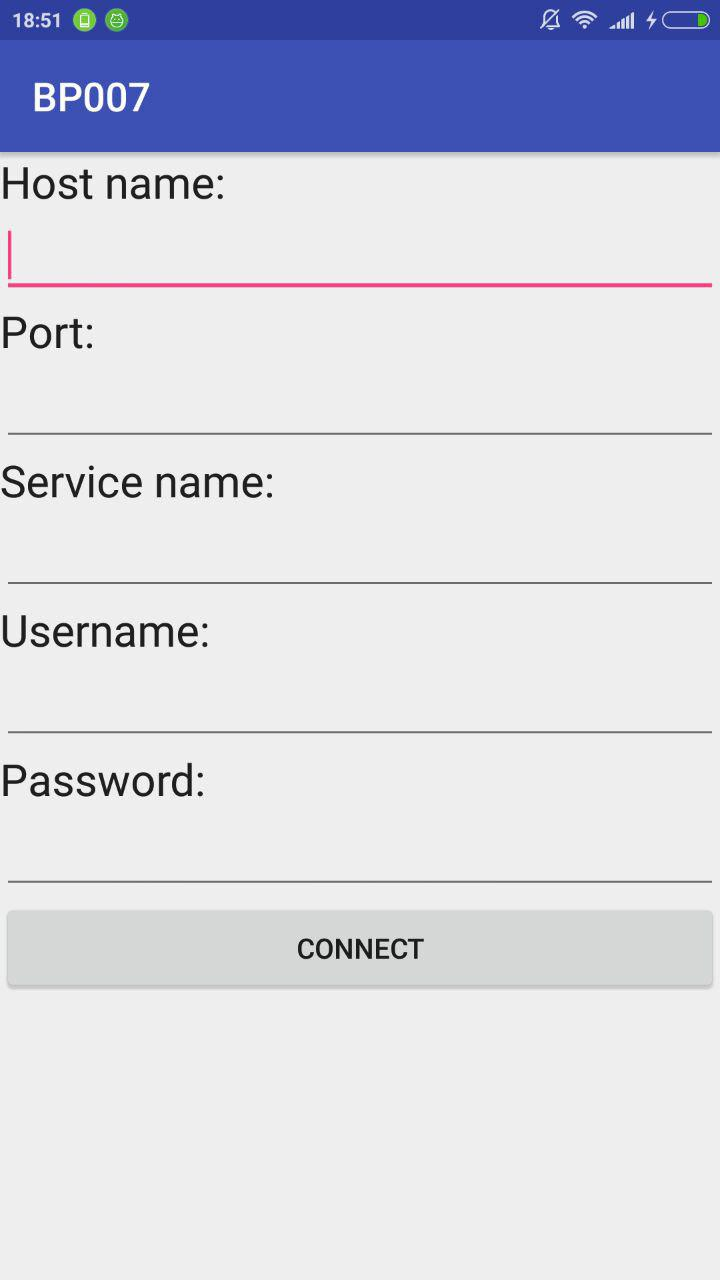
\includegraphics[height=0.5\textwidth]{a.jpg}
	\end{center}
	\caption{Početna aktivnost}
\end{figure}
\newpage
Nakon unosa odgovarajućih podataka, pritisnemo dugme za prijavu:
\begin{figure}[H]
	\begin{center} 
		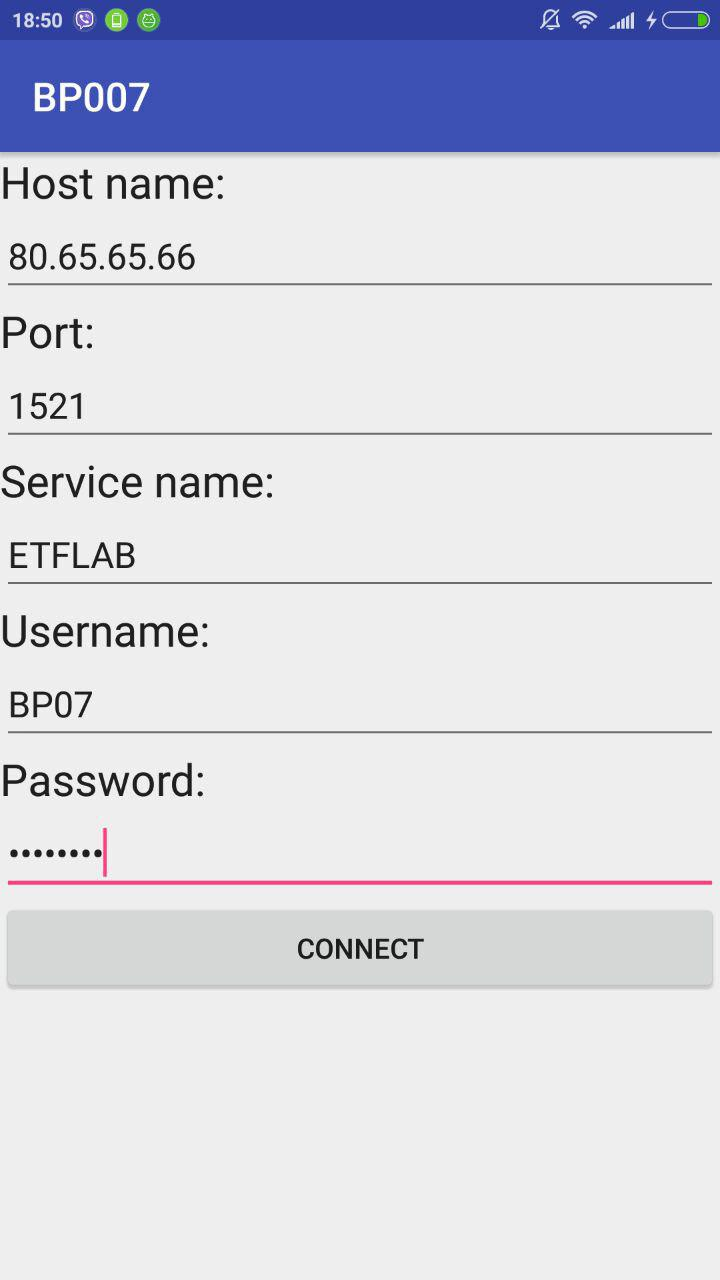
\includegraphics[height=0.5\textwidth]{b.jpg}
	\end{center}
	\caption{Početna aktivnost nakon unosa podataka}
\end{figure}

Nakon uspješne prijave, prelazi se u novu aktivnost na kojoj je prikazana lista objekata baze. U slučaju neuspjeha prikaže se poruka o grešci.
\begin{figure}[H]
	\begin{center} 
		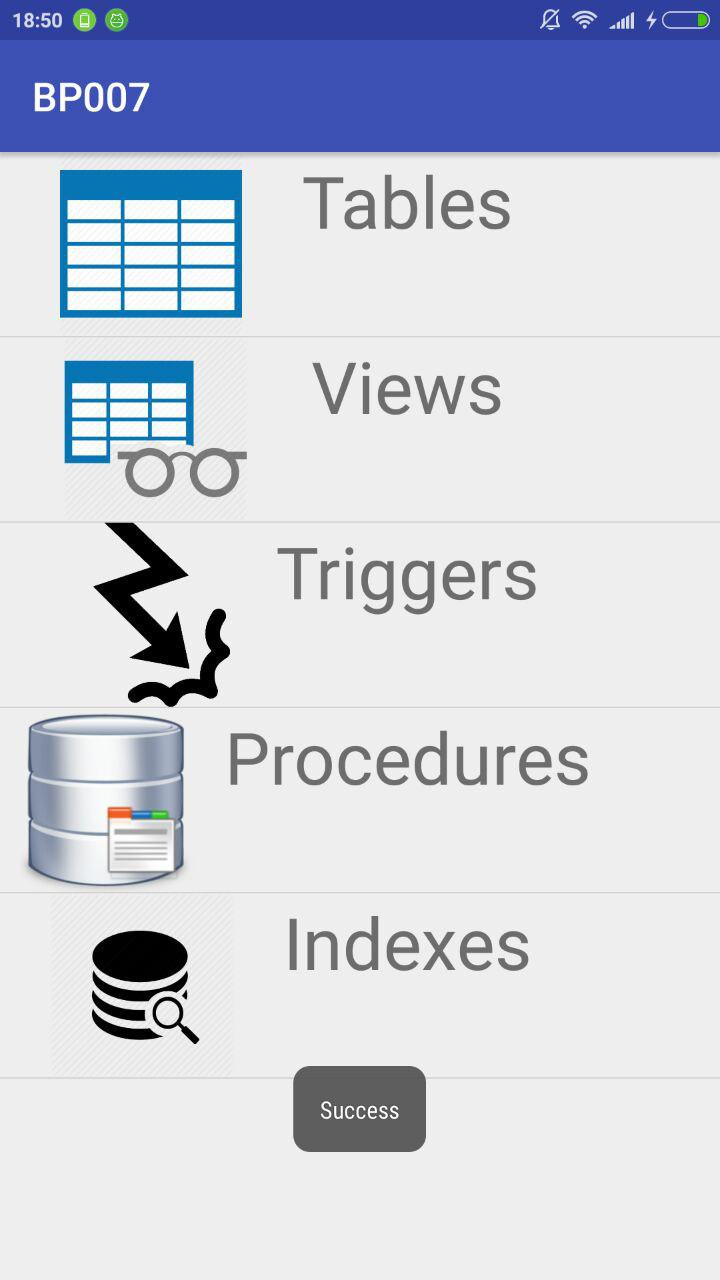
\includegraphics[height=0.5\textwidth]{c.jpg}
	\end{center}
	\caption{Lista objekata baze}
\end{figure}
\newpage
Nakon odabira opcije Tables, prikazuje se lista istih.
\begin{figure}[H]
	\begin{center} 
		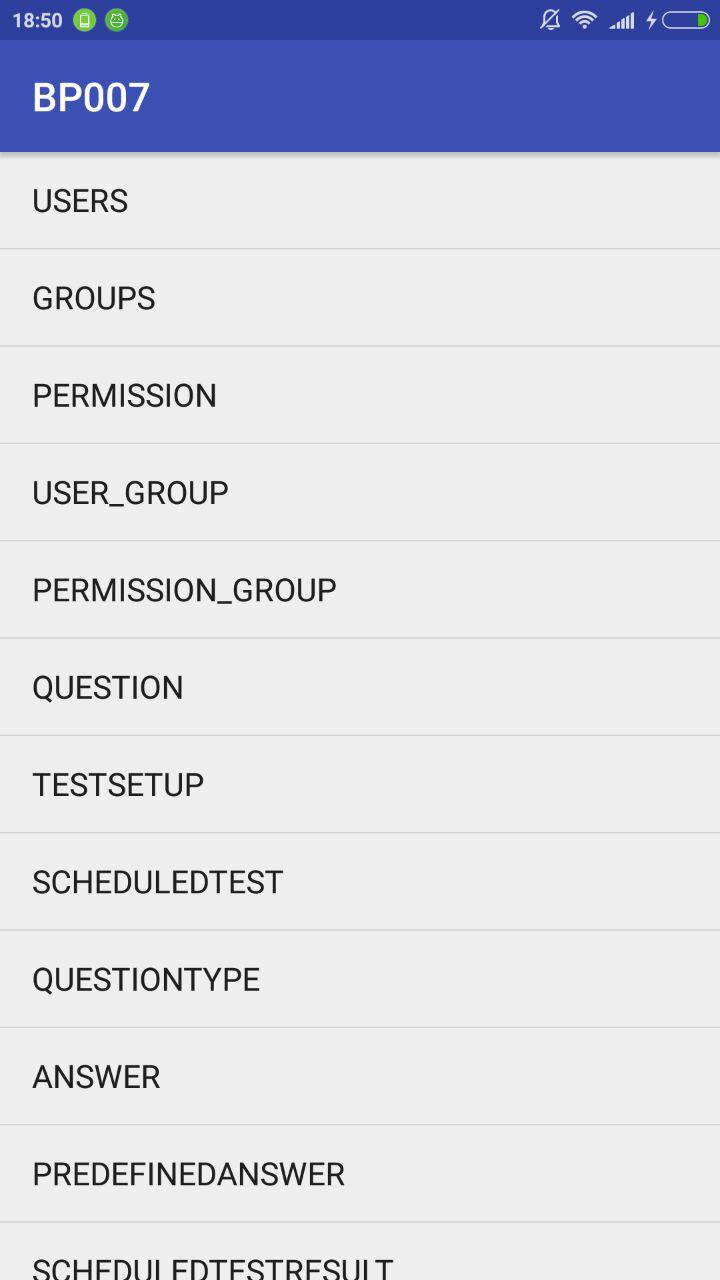
\includegraphics[height=0.5\textwidth]{d.jpg}
	\end{center}
	\caption{Lista tabela}
\end{figure}

Nakon odabira tabele otvara se nova aktivnost na kojoj su prikazani detalji o tabele.
\begin{figure}[H]
	\begin{center} 
		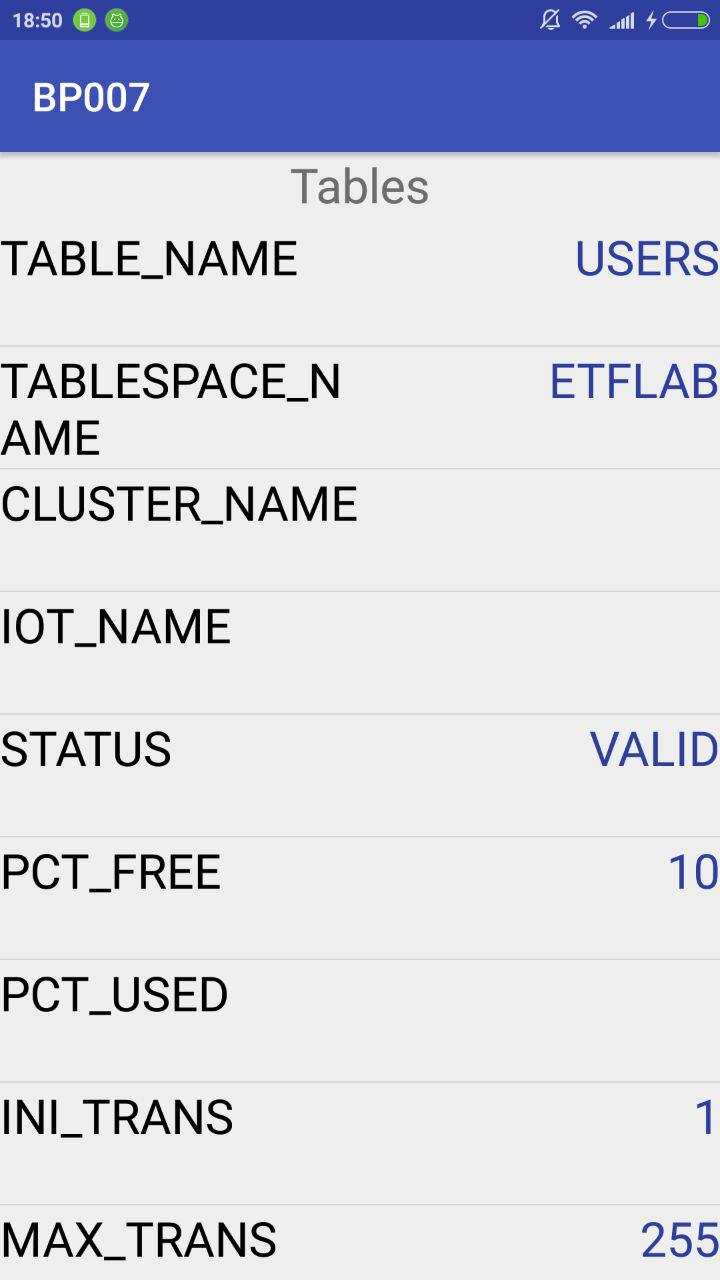
\includegraphics[height=0.5\textwidth]{e.jpg}
	\end{center}
	\caption{Prikaz detalja odabrane tabele}
\end{figure}
\newpage
Nakon odabira opcije Views, prikazuje se lista istih.
\begin{figure}[H]
	\begin{center} 
		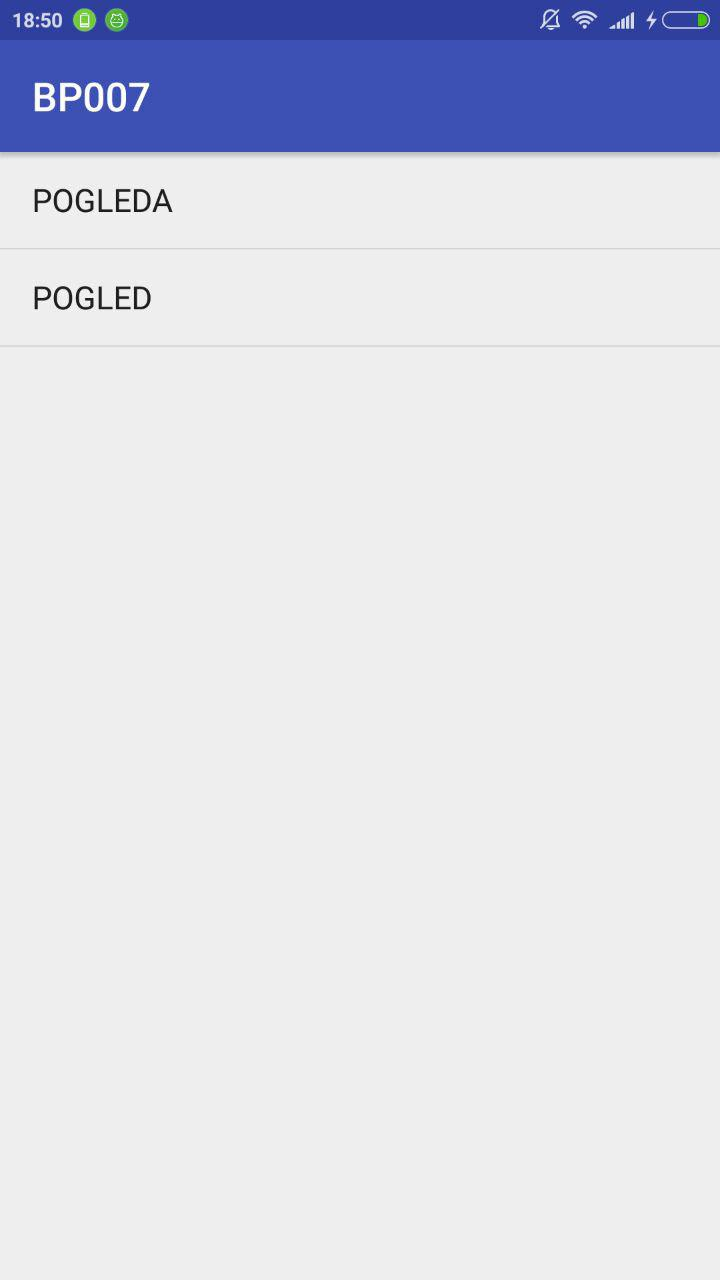
\includegraphics[height=0.5\textwidth]{f.jpg}
	\end{center}
	\caption{Lista pogleda}
\end{figure}

Nakon odabira pogleda otvara se nova aktivnost na kojoj su prikazani detalji o pogledu.
\begin{figure}[H]
	\begin{center} 
		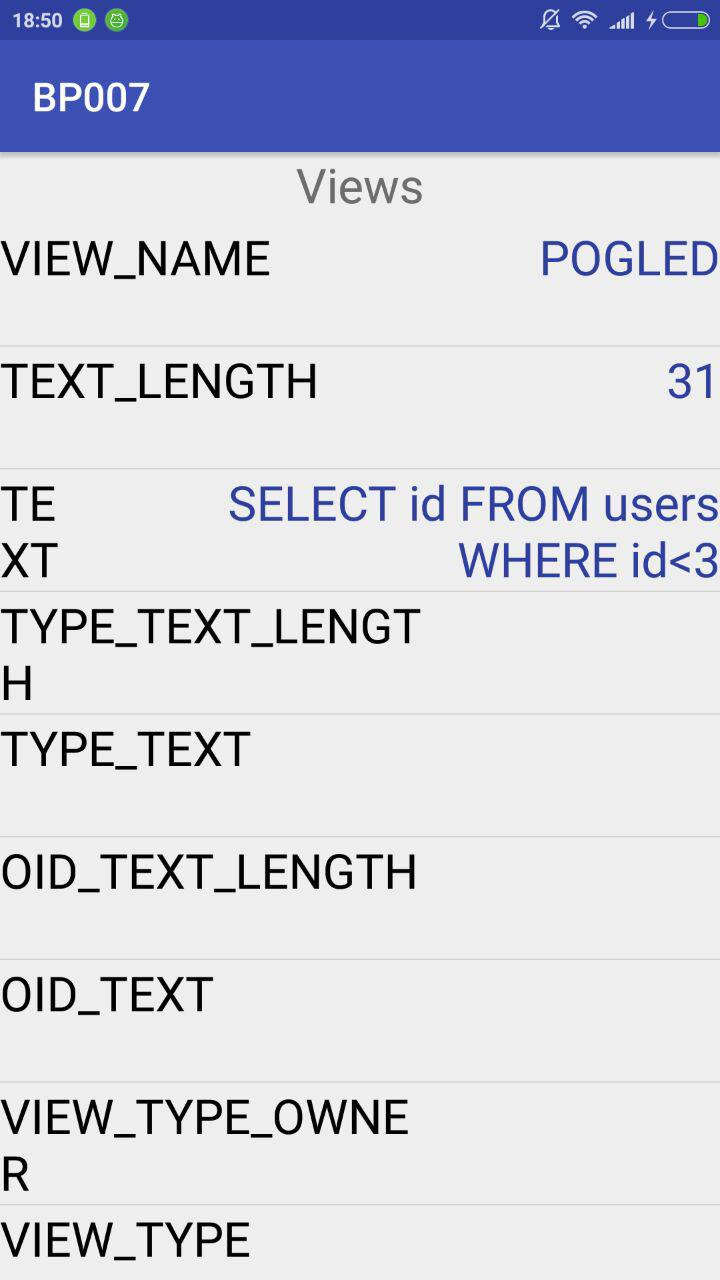
\includegraphics[height=0.5\textwidth]{g.jpg}
	\end{center}
	\caption{Prikaz detalja odabranog pogleda}
\end{figure}
\newpage
Nakon odabira opcije Triggers, prikazuje se lista istih.
\begin{figure}[H]
	\begin{center} 
		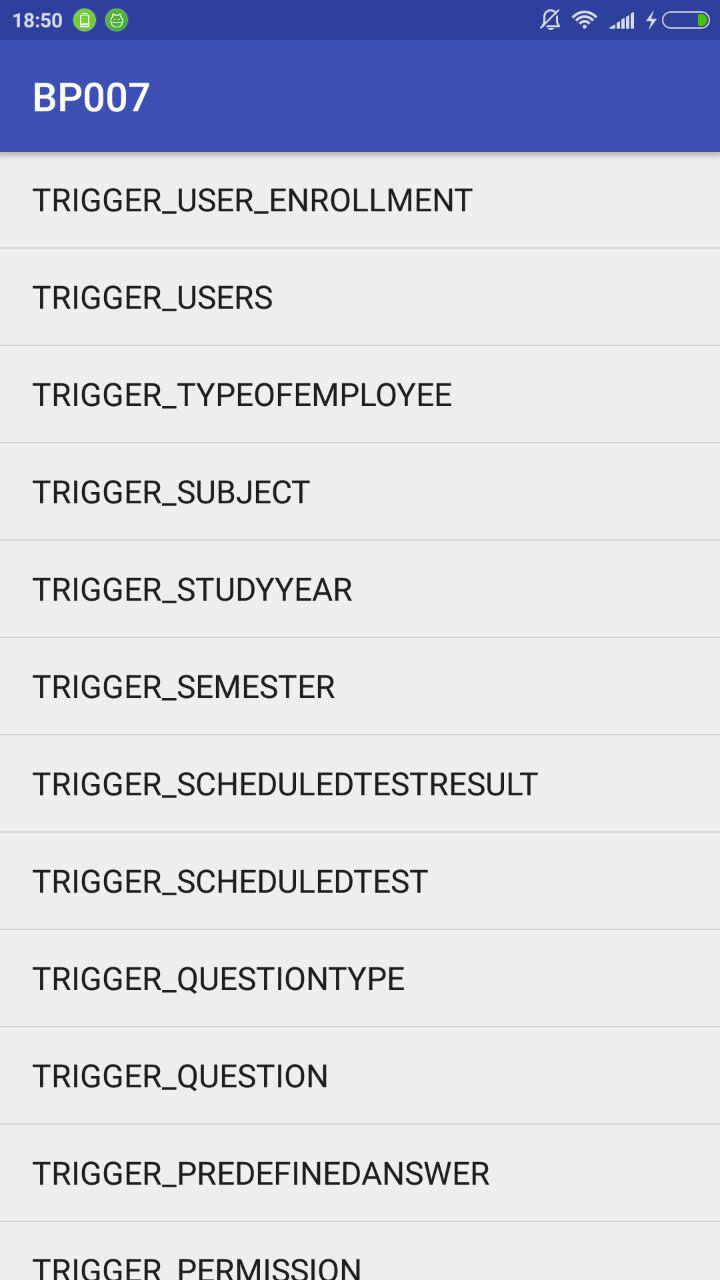
\includegraphics[height=0.5\textwidth]{h.jpg}
	\end{center}
	\caption{Lista triggera}
\end{figure}
Nakon odabira triggera otvara se nova aktivnost na kojoj su prikazani detalji o triggeru.
\begin{figure}[H]
	\begin{center} 
		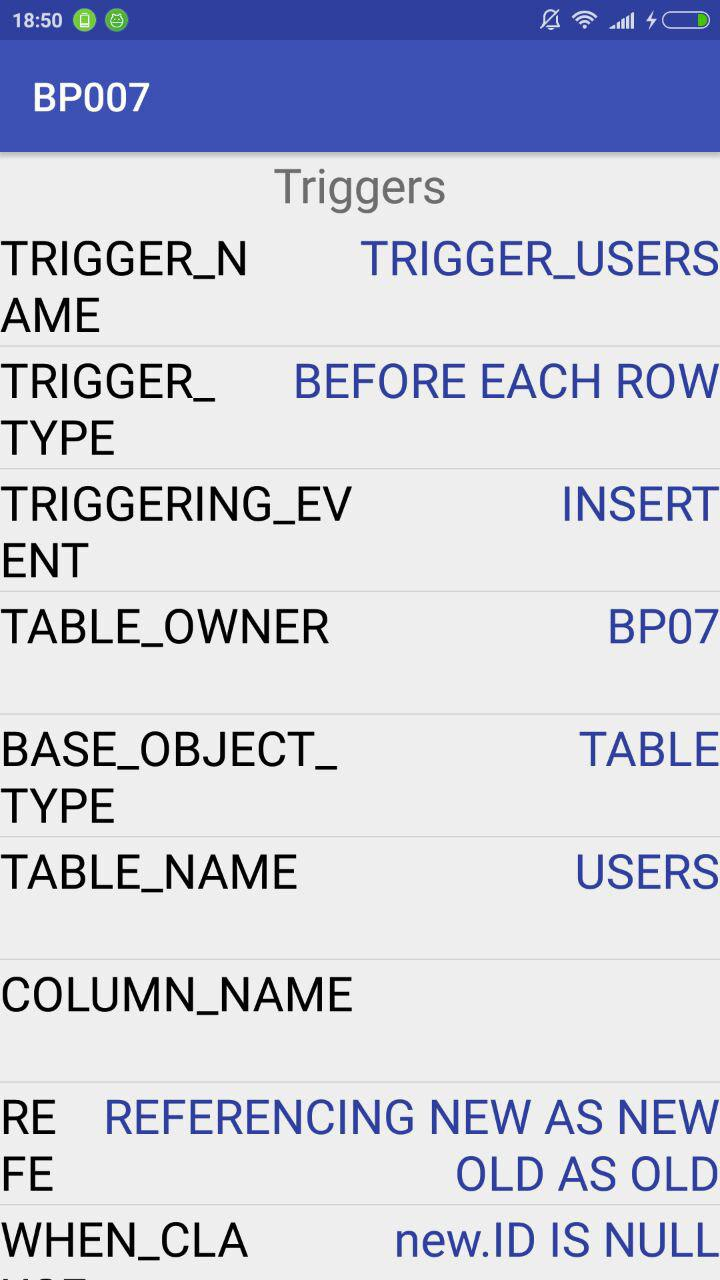
\includegraphics[height=0.5\textwidth]{i.jpg}
	\end{center}
	\caption{Prikaz detalja odabranog triggera}
\end{figure}
\newpage
Nakon odabira opcije Procedures, prikazuje se lista istih.
\begin{figure}[H]
	\begin{center} 
		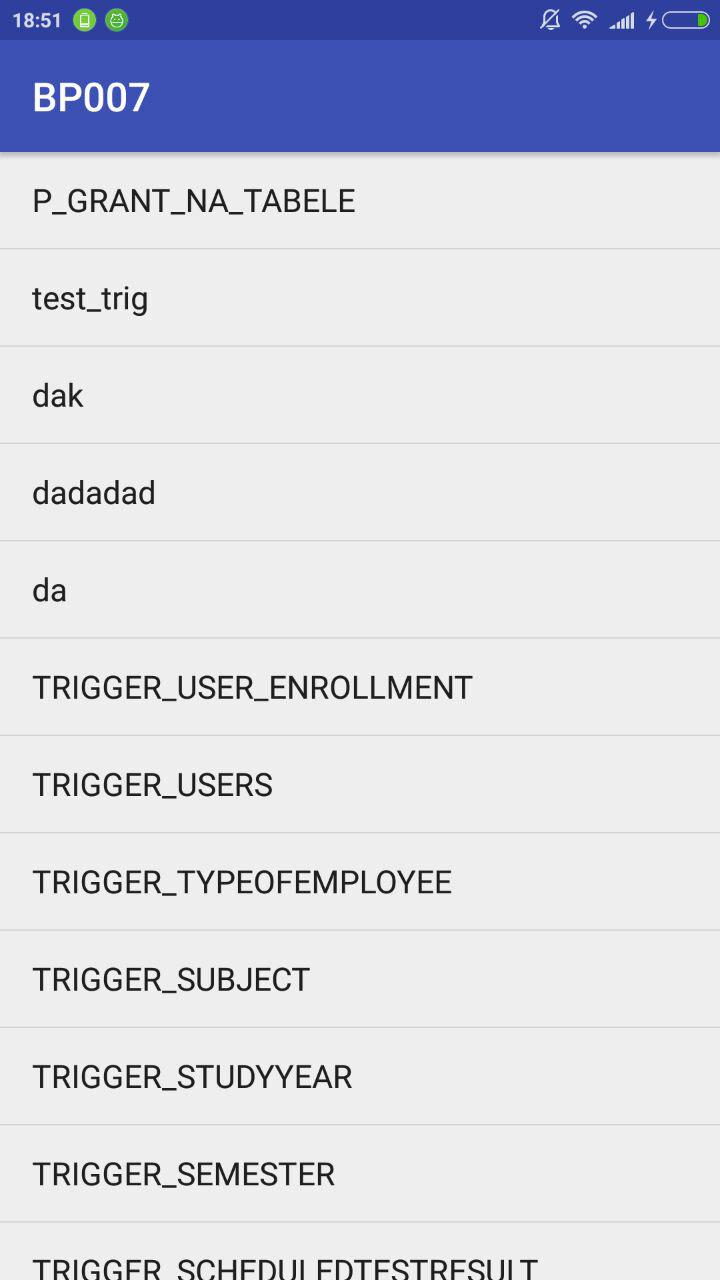
\includegraphics[height=0.5\textwidth]{j.jpg}
	\end{center}
	\caption{Lista procedura}
\end{figure}
Nakon odabira procedure otvara se nova aktivnost na kojoj su prikazani detalji o proceduri.

\begin{figure}[H]
	\begin{center} 
		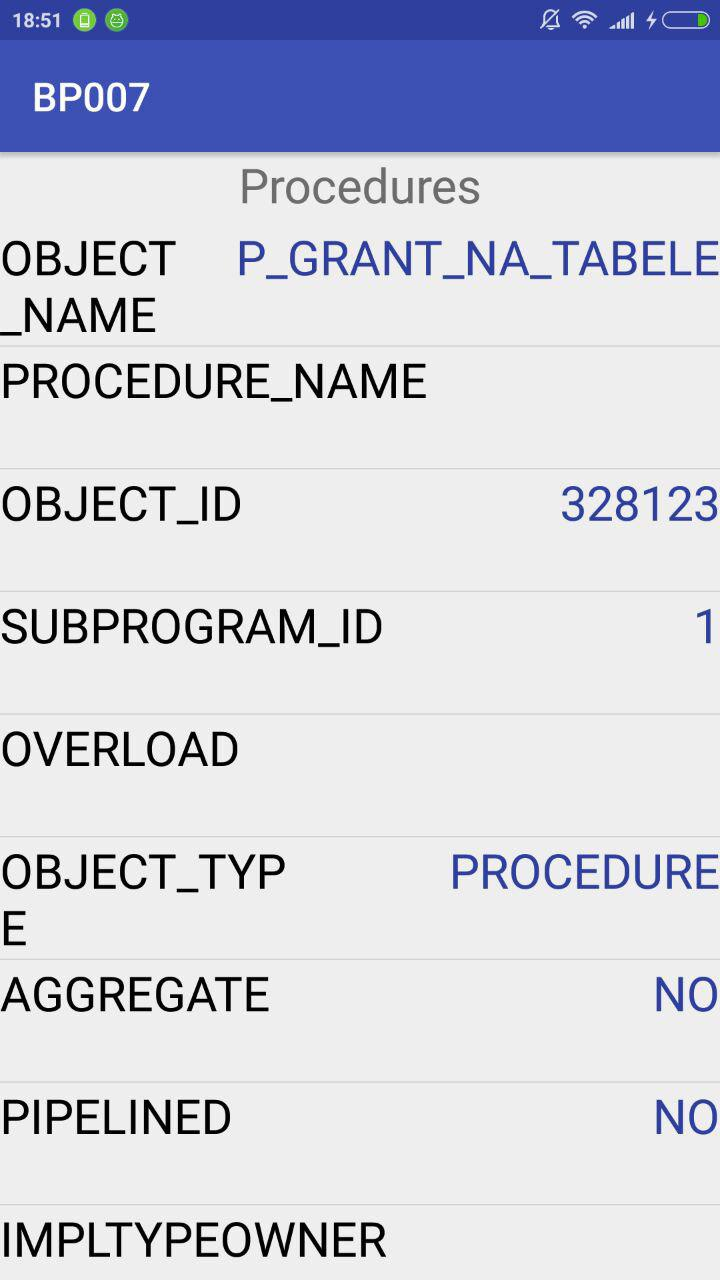
\includegraphics[height=0.5\textwidth]{k.jpg}
	\end{center}
	\caption{Prikaz detalja odabranog procedure}
\end{figure}
\newpage
Nakon odabira opcije Indexes, prikazuje se lista istih.
\begin{figure}[H]
	\begin{center} 
		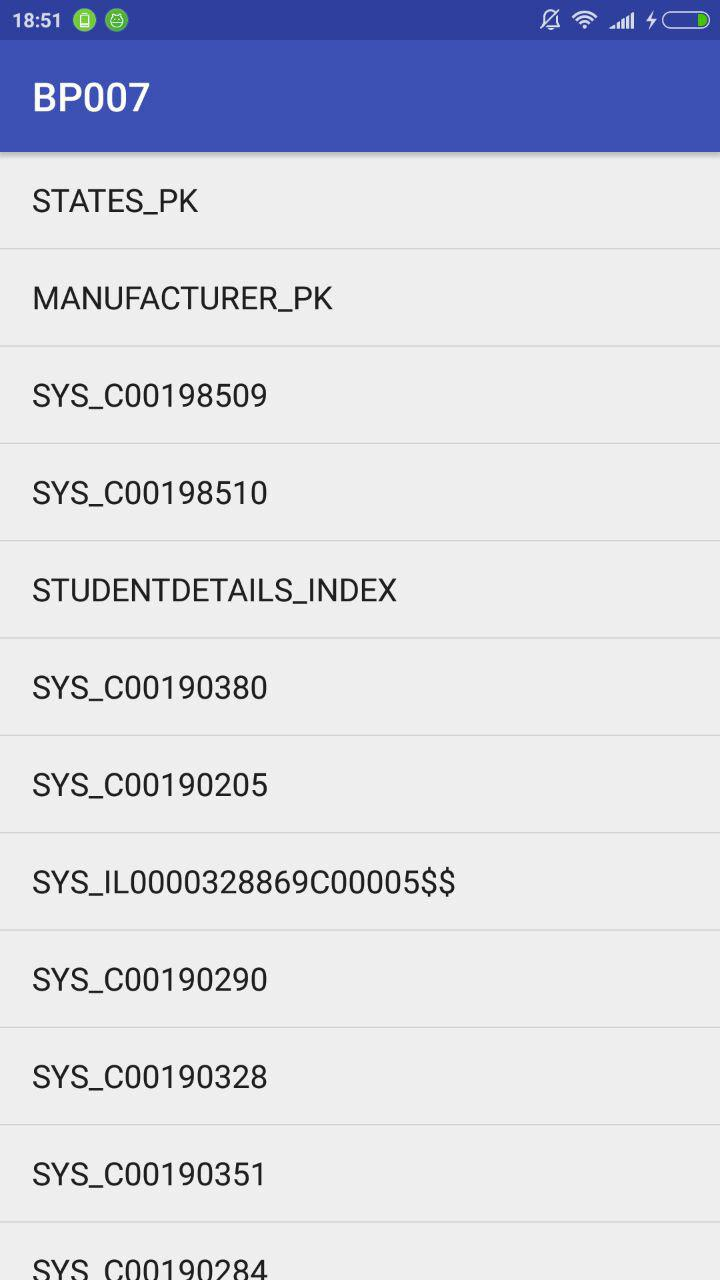
\includegraphics[height=0.5\textwidth]{l.jpg}
	\end{center}
	\caption{Lista indeksa}
\end{figure}

Nakon odabira indeksa otvara se nova aktivnost na kojoj su prikazani detalji o indeksu.
\begin{figure}[H]
	\begin{center} 
		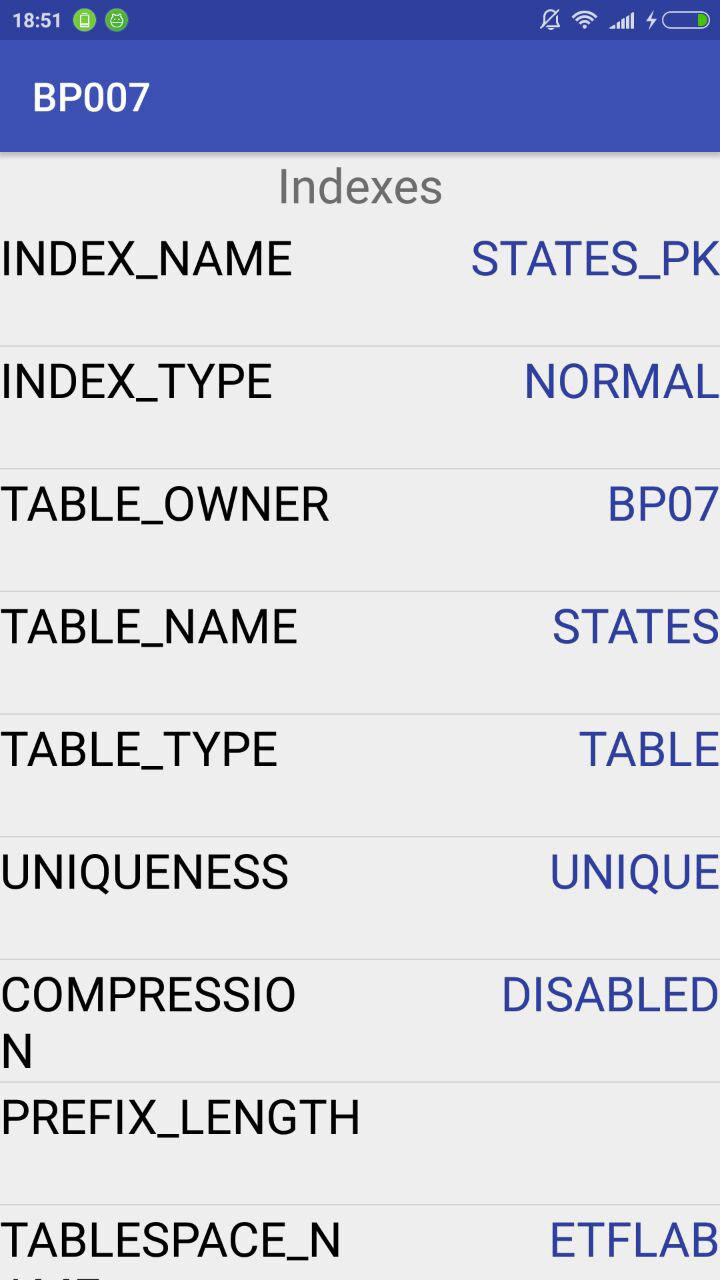
\includegraphics[height=0.5\textwidth]{m.jpg}
	\end{center}
	\caption{Prikaz detalja odabranog indeksa}
\end{figure}



\end{document}